
\documentclass[aspectratio=169,10pt]{beamer}

% ------------------------------------------------------------
% Clean 16:9 Beamer presentation
% Redesigned from the supplied CFD_QAI_chemnitz.pptx
% ------------------------------------------------------------
\usepackage[T1]{fontenc}
\usepackage[utf8]{inputenc}
\usepackage{lmodern}
\usepackage{amsmath,amssymb}
\usepackage{booktabs}
\usepackage{array}
\usepackage{graphicx}
\usepackage{xcolor}
\usepackage{hyperref}
\usepackage{tikz}
\usetikzlibrary{arrows.meta,positioning,fit,calc}

\definecolor{navy}{HTML}{173B4D}
\definecolor{teal}{HTML}{2C6975}
\definecolor{mint}{HTML}{E9F4F2}
\definecolor{orange}{HTML}{D9822B}
\definecolor{lightgray}{HTML}{F3F5F6}
\definecolor{midgray}{HTML}{68757A}
\definecolor{dark}{HTML}{1F2528}

\setbeamercolor{normal text}{fg=dark,bg=white}
\setbeamercolor{structure}{fg=teal}
\setbeamercolor{frametitle}{fg=navy,bg=white}
\setbeamercolor{title}{fg=navy}
\setbeamercolor{subtitle}{fg=midgray}
\setbeamercolor{author}{fg=midgray}
\setbeamercolor{footline}{fg=midgray,bg=white}
\setbeamercolor{block title}{fg=white,bg=navy}
\setbeamercolor{block body}{fg=dark,bg=lightgray}

\setbeamertemplate{navigation symbols}{}
\setbeamertemplate{itemize item}{\color{teal}\small$\blacktriangleright$}
\setbeamertemplate{itemize subitem}{\color{orange}\scriptsize$\blacktriangleright$}

\setbeamertemplate{frametitle}{
  \vspace{0.25cm}
  \begin{beamercolorbox}[wd=\paperwidth,leftskip=0.65cm,rightskip=0.65cm]{frametitle}
    \usebeamerfont{frametitle}\insertframetitle
    \vspace{0.08cm}\par
    {\color{orange}\rule{0.65cm}{1.6pt}}
  \end{beamercolorbox}
}

\setbeamertemplate{footline}{
  \leavevmode
  \hbox{
    \begin{beamercolorbox}[wd=.82\paperwidth,ht=0.35cm,dp=0.15cm,leftskip=.65cm]{footline}
      \scriptsize Combining quantum and physics-inspired AI for CFD
    \end{beamercolorbox}
    \begin{beamercolorbox}[wd=.18\paperwidth,ht=0.35cm,dp=0.15cm,rightskip=.65cm plus1fil]{footline}
      \scriptsize\insertframenumber
    \end{beamercolorbox}
  }
}

\newcommand{\source}[1]{\vspace{0.06cm}{\scriptsize\color{midgray}Source: #1}}
\newcommand{\key}[1]{\textcolor{teal}{\textbf{#1}}}
\newcommand{\highlight}[1]{\textcolor{orange}{\textbf{#1}}}

\title{\textbf{Combining Quantum with Physics-Inspired AI}\\[2mm]
       \textbf{for Accelerating CFD Simulations}}
\subtitle{From physics-informed learning to hybrid quantum--classical CFD}
\author{A Seshaditya}
\institute{QuaSi}
\date{}

\begin{document}

% ------------------------------------------------------------
\begin{frame}[plain]
  \begin{tikzpicture}[remember picture,overlay]
    \fill[navy] (current page.south west) rectangle (current page.north east);
    \fill[teal] (current page.south east) rectangle
      ([xshift=-0.20\paperwidth]current page.north east);
    \fill[orange] ([xshift=-0.20\paperwidth]current page.south east) rectangle
      ([xshift=-0.195\paperwidth]current page.north east);
  \end{tikzpicture}
  \vspace{0.9cm}
  \begin{minipage}{0.76\textwidth}
    {\color{white}\fontsize{25}{30}\selectfont\bfseries
      Combining Quantum with\\Physics-Inspired AI\\[3mm]
      for Accelerating CFD Simulations\par}
    \vspace{0.45cm}
    {\color{white!80}\large From PINNs and neural operators to hybrid quantum--classical models\par}
    \vfill
    {\color{white}\large A Seshaditya\\[1mm]QuaSi\par}
  \end{minipage}
\end{frame}

% ------------------------------------------------------------
\begin{frame}{The problem: CFD is accurate, but expensive}
\begin{columns}[T,onlytextwidth]
\column{0.50\textwidth}
\begin{block}{Why accelerate?}
\begin{itemize}
  \item High computational cost of high-fidelity CFD.
  \item Expensive parameter sweeps and repeated design iterations.
  \item Multi-physics coupling increases model and training complexity.
\end{itemize}
\end{block}
\vspace{0.25cm}
\key{Goal:} learn useful solution structure while retaining the governing physics.

\column{0.47\textwidth}
\centering
\includegraphics[width=\linewidth,height=0.54\textheight,keepaspectratio]{images/image39.png}
\source{Silicon crystal-growth process schematic; source material in supplied deck.}
\end{columns}
\end{frame}

% ------------------------------------------------------------
\begin{frame}{Application focus: two demanding CFD settings}
\begin{columns}[T,onlytextwidth]
\column{0.49\textwidth}
\begin{block}{Silicon crystal growth}
\begin{itemize}
  \item Czochralski (CZ) process.
  \item Coupled Navier--Stokes, particle transport and heat transfer.
  \item Strong thermal--fluid interaction.
\end{itemize}
\centering
\includegraphics[width=.82\linewidth,height=.32\textheight,keepaspectratio]{images/image36.png}
\end{block}

\column{0.49\textwidth}
\begin{block}{Cryogenic / hydrogen systems}
\begin{itemize}
  \item Design-oriented CFD for complex flow and thermal conditions.
  \item Faster surrogate models can support iterative design.
  \item Relevant to the broader space and energy use cases in the source deck.
\end{itemize}
\centering
\includegraphics[width=.82\linewidth,height=.32\textheight,keepaspectratio]{images/image8.png}
\end{block}
\end{columns}
\end{frame}

% ------------------------------------------------------------
\begin{frame}{The technical story}
\centering
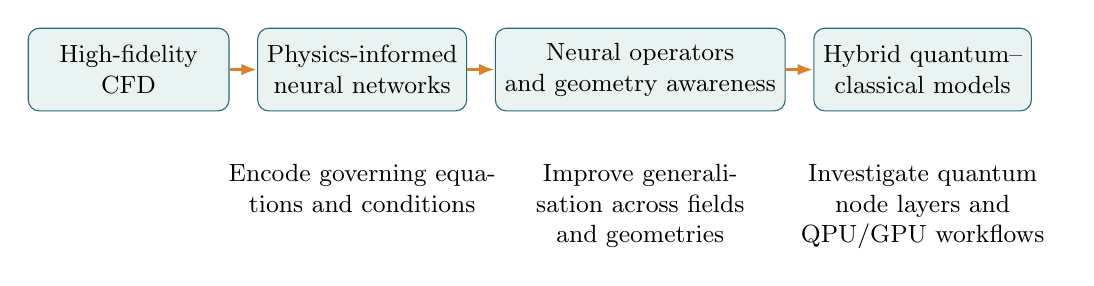
\begin{tikzpicture}[
  node distance=0.55cm and 0.35cm,
  box/.style={rounded corners,draw=teal,fill=mint,minimum width=2.55cm,
              minimum height=1.05cm,align=center,font=\small},
  arr/.style={-{Latex[length=2mm]},very thick,draw=orange}
]
\node[box] (cfd) {High-fidelity\\CFD};
\node[box,right=of cfd] (pinn) {Physics-informed\\neural networks};
\node[box,right=of pinn] (op) {Neural operators\\and geometry awareness};
\node[box,right=of op] (q) {Hybrid quantum--\\classical models};
\draw[arr] (cfd)--(pinn);
\draw[arr] (pinn)--(op);
\draw[arr] (op)--(q);
\node[below=0.55cm of pinn,align=center,text width=3.4cm,font=\small]
{Encode governing equations and conditions};
\node[below=0.55cm of op,align=center,text width=3.4cm,font=\small]
{Improve generalisation across fields and geometries};
\node[below=0.55cm of q,align=center,text width=3.4cm,font=\small]
{Investigate quantum node layers and QPU/GPU workflows};
\end{tikzpicture}

\vfill
\key{Research question:} where can hybrid quantum--classical learning add value without discarding the physics structure?
\end{frame}

% ------------------------------------------------------------
\begin{frame}{Physics-Informed Neural Networks (PINNs)}
\begin{columns}[T,onlytextwidth]
\column{0.48\textwidth}
\begin{block}{Core idea}
A neural network approximates the solution field while the loss function penalises violations of the governing PDEs and boundary/initial conditions.
\end{block}
\begin{itemize}
  \item Less dependence on large labelled datasets.
  \item Natural fit for multi-physics equations.
  \item Automatic differentiation provides PDE residuals.
\end{itemize}
\source{\url{https://doi.org/10.1063/5.0226232}}

\column{0.48\textwidth}
\centering
\includegraphics[width=\linewidth,height=.57\textheight,keepaspectratio]{images/image4.png}
\end{columns}
\end{frame}

% ------------------------------------------------------------
\begin{frame}{PINN methodology: physics becomes part of the objective}
\begin{columns}[T,onlytextwidth]
\column{0.52\textwidth}
\[
L_{\mathrm{total}}
=
L_{\mathrm{PDE}}
+
L_{\mathrm{BC}}
+
L_{\mathrm{IC}}
+
\lambda L_{\mathrm{SAL}}
\]

\begin{description}
\item[$L_{\mathrm{PDE}}$] physics-informed residual.
\item[$L_{\mathrm{BC}}$] boundary-condition loss.
\item[$L_{\mathrm{IC}}$] initial-condition loss.
\item[$L_{\mathrm{SAL}}$] sensitivity-analysis term.
\item[$\lambda$] weighting factor.
\end{description}

\vspace{2mm}
\key{Computation:} automated differentiation.

\column{0.45\textwidth}
\centering
\includegraphics[width=\linewidth,height=.62\textheight,keepaspectratio]{images/image41.png}
\end{columns}
\end{frame}

% ------------------------------------------------------------
\begin{frame}{From PINNs to neural operators}
\begin{columns}[T,onlytextwidth]
\column{0.48\textwidth}
\begin{block}{Why move beyond a single solution?}
Neural operators learn mappings between functions rather than only one fixed field. This can improve reuse across parameter settings and related problems.
\end{block}
\begin{itemize}
  \item PINO: physics-inspired neural operators.
  \item Operator learning targets families of PDE solutions.
  \item The source deck emphasises higher accuracy, multi-physics capability and data efficiency.
\end{itemize}

\column{0.48\textwidth}
\centering
\includegraphics[width=\linewidth,height=.58\textheight,keepaspectratio]{images/image12.png}
\source{PINO/physics-informed operator illustration from supplied deck.}
\end{columns}
\end{frame}

% ------------------------------------------------------------
\begin{frame}{Geometry-aware operators: the next generalisation step}
\begin{columns}[T,onlytextwidth]
\column{0.47\textwidth}
\begin{block}{PI-GANO}
Geometry-aware neural operators aim to generalise across PDE parameter representations and geometries.
\end{block}
\source{arXiv:2408.01600v1}

\begin{block}{GAOT / MAGNO}
The deck also introduces Geometry Aware Operator Transformers and multiscale attentional graph neural operators.
\end{block}
\source{arXiv:2505.18781v2}

\column{0.50\textwidth}
\centering
\includegraphics[width=\linewidth,height=.58\textheight,keepaspectratio]{images/image46.png}
\end{columns}
\end{frame}

% ------------------------------------------------------------
\begin{frame}{A compact comparison of the classical approaches}
\small
\begin{tabular}{>{\raggedright\arraybackslash}p{2.7cm} p{3.0cm} p{3.0cm} p{3.0cm}}
\toprule
\textbf{Approach} & \textbf{Primary idea} & \textbf{Strength in the source deck} & \textbf{Open challenge} \\
\midrule
PINN & NN + PDE residuals & Physics constraints, data efficiency & Training stability and scaling \\
PINO & Operator learning + physics & Families of PDE solutions & Generalisation across settings \\
PI-GANO & Geometry-aware operator & Geometry generalisation & Complex geometries / representations \\
GAOT & Geometry-aware transformer & Attention-based operator learning & Computational cost and validation \\
\bottomrule
\end{tabular}

\vspace{0.35cm}
\centering
\includegraphics[width=.66\linewidth,height=.25\textheight,keepaspectratio]{images/image10.png}

\source{Comparison material in supplied deck; source references include arXiv:2408.01600v1 and arXiv:2505.18781v2.}
\end{frame}

% ------------------------------------------------------------
\begin{frame}{Case study: silicon crystal growth}
\begin{columns}[T,onlytextwidth]
\column{0.50\textwidth}
\begin{block}{Czochralski (CZ) process}
The supplied material frames the problem as a coupled thermal--fluid system involving:
\begin{itemize}
  \item Navier--Stokes equations,
  \item particle transport,
  \item heat transfer.
\end{itemize}
\end{block}
\source{\url{https://doi.org/10.1063/5.0271778}}

\begin{block}{PINN role}
Parameter sensitivity is highlighted for temperature gradients, precursor pressure/concentrations, flow rates and substrate properties.
\end{block}

\column{0.47\textwidth}
\centering
\includegraphics[width=\linewidth,height=.63\textheight,keepaspectratio]{images/image17.png}
\end{columns}
\end{frame}

% ------------------------------------------------------------
\begin{frame}{Improving the PINN for thermal--fluid coupling}
\begin{columns}[T,onlytextwidth]
\column{0.46\textwidth}
\begin{block}{Spatial information + adaptive loss balance}
The source deck describes an approach intended to:
\begin{itemize}
  \item optimise thermal--fluid coupling,
  \item improve training stability,
  \item balance contributions from different physics terms.
\end{itemize}
\end{block}
\source{\url{https://doi.org/10.1063/5.0271778}}

\column{0.51\textwidth}
\centering
\includegraphics[width=\linewidth,height=.58\textheight,keepaspectratio]{images/image42.png}
\vspace{1mm}
\scriptsize Representative simulation/result material from the supplied presentation.
\end{columns}
\end{frame}

% ------------------------------------------------------------
\begin{frame}{Why bring quantum computing into the workflow?}
\begin{columns}[T,onlytextwidth]
\column{0.48\textwidth}
\begin{block}{Hybrid rather than replacement}
The proposed direction is to combine classical physics-informed models with quantum components, using QPU/GPU hardware where appropriate.
\end{block}

\begin{itemize}
  \item Quantum node layers inside otherwise classical architectures.
  \item Variational quantum circuits (VQCs).
  \item Exploration of quantum neural operators and quantum-enhanced PINNs.
\end{itemize}

\column{0.49\textwidth}
\centering
\includegraphics[width=\linewidth,height=.57\textheight,keepaspectratio]{images/image48.png}
\source{Hybrid quantum--classical PINN architecture; source: arXiv:2304.11247v3.}
\end{columns}
\end{frame}

% ------------------------------------------------------------
\begin{frame}{Quantum PINNs: candidate architectures}
\begin{columns}[T,onlytextwidth]
\column{0.49\textwidth}
\begin{block}{Quantum node layer}
A quantum layer can be embedded into a classical neural architecture, creating a hybrid model rather than a fully quantum solver.
\end{block}
\begin{itemize}
  \item Multi-variational quantum layers.
  \item Classical layers surrounding quantum components.
  \item Geometry-focused VQCs.
\end{itemize}
\source{\url{https://www.mdpi.com/1099-4300/26/8/649}}

\column{0.48\textwidth}
\centering
\includegraphics[width=\linewidth,height=.56\textheight,keepaspectratio]{images/image49.png}
\source{Quantum-node / variational-circuit architecture from supplied deck.}
\end{columns}
\end{frame}

% ------------------------------------------------------------
\begin{frame}{Quantum operators and attention-enhanced models}
\begin{columns}[T,onlytextwidth]
\column{0.48\textwidth}
\begin{block}{Quantum DeepONets}
The deck points to quantum-enhanced operator learning as a route toward neural operators accelerated by quantum computing.
\end{block}
\source{\url{https://arxiv.org/pdf/2409.15683}}

\begin{block}{Attention-enhanced QPINNs}
Attention mechanisms and tensor-network ideas are also presented as candidate routes for improving expressive capacity.
\end{block}

\column{0.49\textwidth}
\centering
\includegraphics[width=\linewidth,height=.56\textheight,keepaspectratio]{images/image25.png}
\end{columns}
\end{frame}

% ------------------------------------------------------------
\begin{frame}{Where quantum advantage is—and is not—established}
\begin{block}{Important distinction}
The supplied presentation treats quantum advantage as a \highlight{research objective}, not as an established result for general CFD.
\end{block}

\begin{columns}[T,onlytextwidth]
\column{0.49\textwidth}
\textbf{What is demonstrated or proposed}
\begin{itemize}
  \item Hybrid quantum/classical architectures.
  \item Quantum node layers and VQCs.
  \item Candidate PDE and CFD applications.
  \item Reduced training-data requirements are discussed for specific case studies.
\end{itemize}

\column{0.49\textwidth}
\textbf{What still needs benchmarking}
\begin{itemize}
  \item Wall-clock time versus strong classical baselines.
  \item End-to-end cost including QPU access and data movement.
  \item Accuracy across geometry and parameter changes.
  \item Reproducibility on realistic CFD workloads.
\end{itemize}
\end{columns}

\vspace{2mm}
\source{QCPINN case study: arXiv:2503.16678; supplied deck notes a potential 80--90\% reduction in training volume for that study.}
\end{frame}

% ------------------------------------------------------------
\begin{frame}{Implementation: connect QPU and HPC/GPU resources}
\begin{columns}[T,onlytextwidth]
\column{0.47\textwidth}
\begin{block}{Software / hardware ecosystem shown in the deck}
\begin{itemize}
  \item PennyLane
  \item NVIDIA Modulus
  \item DGX Quantum
  \item IBM Quantum
\end{itemize}
\end{block}

\begin{block}{Workflow principle}
Keep the expensive, highly parallel CFD and neural-network operations on classical HPC/GPU infrastructure, while testing quantum components where they can be isolated and benchmarked.
\end{block}

\column{0.50\textwidth}
\centering
\includegraphics[width=\linewidth,height=.58\textheight,keepaspectratio]{images/image29.png}
\source{QC--HPC integration architecture; source: arXiv:2408.16159v1.}
\end{columns}
\end{frame}

% ------------------------------------------------------------
\begin{frame}{A practical research and validation roadmap}
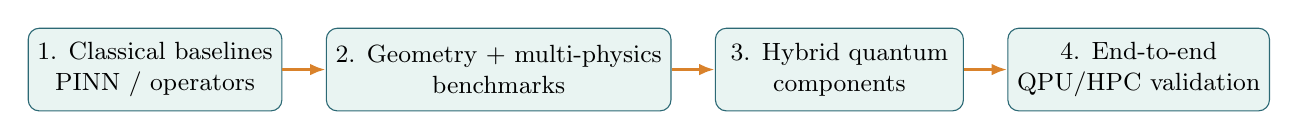
\begin{tikzpicture}[
  node distance=0.55cm,
  roadmapstep/.style={rounded corners,draw=teal,fill=mint,minimum width=3.15cm,
               minimum height=1.05cm,align=center,font=\small},
  arr/.style={-{Latex[length=2mm]},very thick,draw=orange}
]
\node[roadmapstep] (s1) {1. Classical baselines\\PINN / operators};
\node[roadmapstep,right=0.55cm of s1] (s2) {2. Geometry + multi-physics\\benchmarks};
\node[roadmapstep,right=0.55cm of s2] (s3) {3. Hybrid quantum\\components};
\node[roadmapstep,right=0.55cm of s3] (s4) {4. End-to-end\\QPU/HPC validation};
\draw[arr] (s1)--(s2);
\draw[arr] (s2)--(s3);
\draw[arr] (s3)--(s4);
\end{tikzpicture}

\vspace{0.45cm}
\begin{columns}[T,onlytextwidth]
\column{0.49\textwidth}
\textbf{Benchmark dimensions}
\begin{itemize}
  \item Accuracy and conservation properties.
  \item Training/inference time.
  \item Data and memory requirements.
\end{itemize}

\column{0.49\textwidth}
\textbf{Validation settings}
\begin{itemize}
  \item Silicon crystal growth.
  \item Turbulent-flow examples.
  \item Cryogenic / CFRP vessel examples referenced in the source deck.
\end{itemize}
\end{columns}
\end{frame}

% ------------------------------------------------------------
\begin{frame}{Outlook: from promising components to validated CFD workflows}
\begin{columns}[T,onlytextwidth]
\column{0.50\textwidth}
\begin{block}{Near-term}
\begin{itemize}
  \item Benchmark physics- and geometry-aware AI models.
  \item Compare hybrid quantum models against strong classical baselines.
  \item Quantify where quantum components change the accuracy/cost trade-off.
\end{itemize}
\end{block}

\column{0.47\textwidth}
\begin{block}{Longer-term}
\begin{itemize}
  \item QPU/GPU integrated simulation pipelines.
  \item Academic and industrial collaborations.
  \item Pilot projects for aerospace and related engineering applications.
\end{itemize}
\end{block}
\end{columns}

\vfill
\centering
\includegraphics[width=.46\linewidth,height=.20\textheight,keepaspectratio]{images/image60.png}

\key{Core message:} physics-informed learning provides the foundation; geometry-aware operators improve reuse; hybrid quantum models are the next hypothesis to test.
\end{frame}

% ------------------------------------------------------------
\begin{frame}{Key takeaways}
\begin{enumerate}
  \item \key{CFD acceleration is the driver:} high-fidelity multi-physics simulations are computationally expensive.
  \item \key{PINNs add physics constraints:} PDEs, boundary conditions and initial conditions become part of learning.
  \item \key{Operators add generalisation:} PINO, PI-GANO and GAOT target mappings across solution families and geometries.
  \item \key{Quantum is a hybrid research direction:} QPINNs, quantum node layers and quantum operators can be tested within classical workflows.
  \item \key{Validation is essential:} claims of quantum advantage need end-to-end, problem-specific benchmarking.
\end{enumerate}

\vfill
\centering
\large\textcolor{navy}{Physics + geometry + hybrid quantum resources}\\
\large\textcolor{midgray}{\(\longrightarrow\) a coherent path toward accelerated CFD}
\end{frame}

% ------------------------------------------------------------
\begin{frame}{Selected references from the supplied deck}
\scriptsize
\begin{itemize}
  \item Afrah Farea, Saiful Khan, Mustafa Serdar Celebi (2025), \emph{QCPINN: Quantum-Classical Physics-Informed Neural Networks for Solving PDEs}, arXiv:2503.16678.
  \item \emph{Hybrid Quantum PINNs for Computational Fluid Dynamics} (2025), IOP Science, doi:10.1088/2632-2153/ad43b2.
  \item \emph{Quantum Physics-Informed Machine Learning for Multiscale Simulations} (2024), arXiv:2403.08954.
  \item \emph{PINNSFORMER: A Transformer-Based Framework for Physics-Informed Neural Networks} (2023), arXiv:2307.11833v3.
  \item Pengpeng Xiao et al. (2024), \emph{Quantum DeepONet: Neural Operators Accelerated by Quantum Computing}, manuscript.
  \item Siddhant Dutta et al. (2024), \emph{AQ-PINNs: Attention-Enhanced Quantum Physics-Informed Neural Networks for Carbon-Efficient Climate Modeling}, arXiv:2409.01626.
  \item D. Kolberg, C. Anders, S. Reke (2023), silicon VMCz crystal-growth PINNs, doi:10.1080/00219592.2023.2236656.
  \item J. Ling, Y. Zhang, D. Chen (2023), thermal-fluid coupling in silicon crystal growth, doi:10.1063/5.0123811.
  \item Y. Zhao, H. Liu, J. Xu (2025), thermal-fluid coupling in Czochralski silicon growth, doi:10.1063/5.0271778.
\end{itemize}
\end{frame}

% ------------------------------------------------------------
\begin{frame}[plain]
\begin{tikzpicture}[remember picture,overlay]
  \fill[navy] (current page.south west) rectangle (current page.north east);
  \fill[teal] (current page.south east) rectangle
    ([xshift=-0.20\paperwidth]current page.north east);
  \fill[orange] ([xshift=-0.20\paperwidth]current page.south east) rectangle
    ([xshift=-0.195\paperwidth]current page.north east);
\end{tikzpicture}
\vspace{1.0cm}
{\color{white}\fontsize{30}{36}\selectfont\bfseries Thank you\par}
\vspace{0.35cm}
{\color{white!85}\large A Seshaditya\par}
\vspace{0.1cm}
{\color{white!75}\normalsize
\href{https://quasi.digital}{quasi.digital}\\
\href{https://github.com/adytiaa/quasi.ai}{github.com/adytiaa/quasi.ai}\\
\href{https://adytiaa.github.io/quasi.ai/}{adytiaa.github.io/quasi.ai/}\par}
\vfill
{\color{white!65}\small Combining Quantum with Physics-Inspired AI Models for Accelerating CFD Simulations\par}
\end{frame}

\end{document}
